\documentclass{standalone}

\usepackage{pgfplots,tikz,amsmath}
\begin{document}
            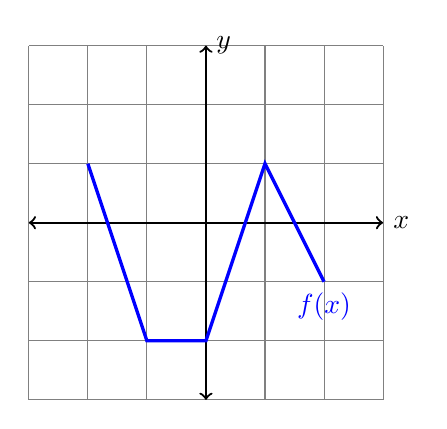
\begin{tikzpicture}[scale=0.75]
                \draw[color=gray] (-3,-3) grid (3,3);
                \draw[thick, black, <->] (-3,0) -- (3,0) node[anchor=west]{$x$};
                \draw[thick, black, <->] (0,-3) -- (0,3) node[anchor=west]{$y$};
                \draw[very thick, blue] (-2,1) -- (-1,-2) -- (0,-2) -- (1,1) -- (2,-1)
                node[anchor=north]{$f(x)$}; 
            \end{tikzpicture}
            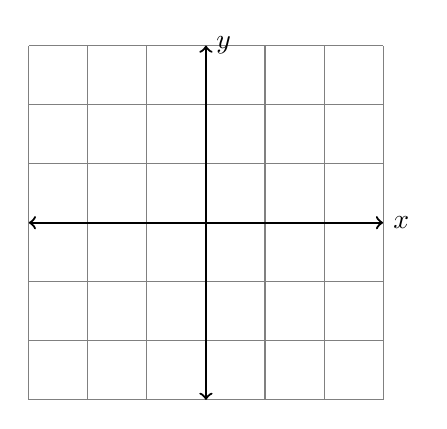
\begin{tikzpicture}[scale=0.75]
                \draw[color=gray] (-3,-3) grid (3,3);
                \draw[thick, black, <->] (-3,0) -- (3,0) node[anchor=west]{$x$};
                \draw[thick, black, <->] (0,-3) -- (0,3) node[anchor=west]{$y$};
            \end{tikzpicture}
\end{document}
